\section{Implementation}
\label{appx:implementation}

\subsection{Overview}
\label{appx:implementation overview}

\paragraph{Training Stage} For rollout generation, we use stochastic sampling with temperature $1.0$ and top-$p=1.0$, which encourages broad exploration of the model's response distribution during RL training. This is important for \method, since the diversity reward can only provide useful learning signal when the sampled response group contains meaningful variation. We sample $k=6$ mode-conditioned responses per prompt, forming the group over which diversity rewards and GRPO advantages are computed. We use a maximum prompt length of $1024$ tokens and a maximum response length of $2048$ tokens. For the Quality Gated Diversity Reward, we used quality weight of $\lambda_q=1$, diversity reward weight of $\lambda_d=100$, length penalty weight of $0.01$, and language-mismatch penalty of weight  $0.1$. For GLM-4-9B base, we observed a severe language-mismatch issue in its response, and therefore increased the weight of the language-mismatch penalty to $100$.

For Qwen3-8B base, we trained \method{} and all baselines for 4 epochs. For Llama-3.1-8B, GLM-4-9B base and ablation models, we trained for 2 epochs due to compute resource constraints.

Our training were performed on NVIDIA A100, H100 or H200 GPUs, depending on availability. A single training for 2 epochs run takes approximately 24 hours on 4 H200 GPUs.
We provide the rest of the training parameters in Table \ref{tab:hyperparameter}.

\begin{table}[t]
\centering
\caption{
Training hyperparameters used for \method{}.
}
\label{tab:training-hyperparams}
\small
\begin{tabular}{ll}
\toprule
\textbf{Hyperparameter} & \textbf{Value} \\
\midrule
\multicolumn{2}{l}{\textit{Model and data}} \\
Base model & Qwen3-8B \\
Training batch size & 32 \\
Validation batch size & 32 \\
Maximum prompt length & 1024 \\
Maximum response length & 2048 \\
Number of training epochs & 2 \\
\midrule
\multicolumn{2}{l}{\textit{Rollout generation}} \\
Rollout engine & vLLM \\
Number of responses per prompt, $N$ & 6 \\
Sampling & Enabled \\
Temperature & 1.0 \\
Top-$p$ & 1.0 \\
Top-$k$ & $-1$ \\
Maximum model length & 4096 \\
\midrule
\multicolumn{2}{l}{\textit{Policy optimization}} \\
RL algorithm & GRPO \\
Actor learning rate & $1\times 10^{-6}$ \\
Optimizer & AdamW \\
AdamW betas & $(0.9, 0.999)$ \\
Weight decay & 0.01 \\
Gradient clipping & 1.0 \\
PPO epochs & 1 \\
PPO mini-batch size & 32 \\
PPO micro-batch size per GPU & 4 \\
PPO clip ratio & 0.2 \\
Advantage normalization & Enabled \\
Loss aggregation & Token mean \\
Entropy coefficient & 0 \\
\midrule
\multicolumn{2}{l}{\textit{KL regularization}} \\
Use KL loss & Enabled \\
KL loss coefficient & 0.01 \\
KL loss type & Low-variance KL \\
KL control coefficient & 0.001 \\
Target KL & 0.1 \\
\midrule
\multicolumn{2}{l}{\textit{Reward function}} \\
Quality reward weight & 1.0 \\
Distinctiveness reward weight & 100.0 \\
Thresholding base reward & 0.5 \\
Length penalty weight & 0.01 \\
Maximum length before penalty & 512 tokens \\
Language mixing penalty weight (Qwen/Llama) & 0.1 \\
Language mixing penalty weight (GLM) & 10 \\
\bottomrule
\end{tabular}
\label{tab:hyperparameter}
\end{table}

\subsection{Ablation Model Implementations}
\label{appx: ablation model implementations}

\textbf{Additive Aggregation.}\label{ablation: additive aggregation} Many existing works on quality-diversity optimization aggregate quality and diversity objectives using a weighted sum~\citep{mouret2015illuminatingsearchspacesmapping, Chen2025PosttrainingLL}. We compare our method with variants trained using an additive reward objective. We find that additive aggregation is highly sensitive to the diversity weight $\lambda_d$. at $\lambda_d=1$, the additive variant shows modest diversity improvement over the baseline, but substantially less than \method{}; at $\lambda_d=10$ and $\lambda_d=100$, diversity improves significantly, but at the cost of general capability performance under diverse decoding. In contrast, \method{} separates quality control from diversity optimization through the quality gate, making the reward less sensitive to coefficient scaling and enables faster iteration.

\textbf{Role Injection.}
\label{ablation: role injection}
Prior work has shown that manually designed prompts can induce different model
behaviors \citep{park2024generative, argyle2023out}. We therefore craft six personas and inject them into the system prompt instead of the abstract numbered roles, testing whether hand-designed personas provide a stronger diversity prior than the abstract numbered role used in the main setting. To isolate the effect of role multiplicity from role content, we train a single-role variant in which every response is generated under the same \textit{``You are Role 1.''} system prompt. To study the effect of the identity-based role, we train a token-based conditioning variant in which the system prompt instructs a token-based distinguishing signal (e.g. \textit{``Start your response with APPLE/BANANA/ORANGE.''}).
As shown in Table~\ref{tab:ablation}, all variants exhibit a slight diversity improvement over the base model, but their gains are smaller than \method{}'s, indicating that multiple abstract numbered identity-based roles provide a more effective exploration space than all the ablated variants, without sacrificing generalization.

\paragraph{Token-based roles}
As an ablation, we replace the abstract numbered role instructions with dummy roles. Specifically, for each prompt, we prepend one of the
following system prompts. We stripped the dummy tokens (e.g., \textit{APPLE}/\textit{ORANGE}/\textit{BANANA}) from the responses before computing the diversity and quality metrics, both during the training and during the evaluation.

\begin{quote}
\small
\begin{enumerate}
    \item ``Start your response with APPLE.''
    \item ``Start your response with ORANGE.''
    \item ``Start your response with BANANA.''
    \item ``Start your response with CHERRY.''
    \item ``Start your response with DATE.''
    \item ``Start your response with ELDERBERRY.''
\end{enumerate}
\end{quote}


\paragraph{Crafted roles}
As an ablation, we replace the abstract numbered role instructions with manually
crafted role descriptions. Specifically, for each prompt, we prepend one of the
following system prompts:
\begin{quote}
\small
\begin{enumerate}
    \item ``You are a helpful assistant.''
    \item ``You are a creative problem solver.''
    \item ``You are a patient educator.''
    \item ``You are a rigorous mathematician.''
    \item ``You are a skeptical analyst.''
    \item ``You are an optimistic encourager.''
\end{enumerate}
\end{quote}

\paragraph{Single role}
As an ablation, we use only one role for mode condition. We prepend ``You are Role 1." on each system prompt.

\subsection{Dataset}
\label{appx:dataset}
Our training dataset comprises a mixture of general-purpose SFT prompts, which anchor baseline capability, and open-ended prompts, which encourage exploration and response diversity. Specifically, we sample 8k prompts from \texttt{allenai/tulu-3-sft-mixture} \citep{lambert2024tulu3} as general-purpose examples and 2k prompts from Infinite-Chat as open-ended queries. We held out a portion of Infinite-Chat for evaluation.

\subsection{Discriminator}
\label{appx:discriminator}
We train a lightweight pairwise binary discriminator to predict whether two responses to the same prompt are conceptually distinct. The training data is constructed from \(2{,}000\) Alpaca~\citep{alpaca} prompts. For each
prompt, we employ Qwen3-30B to generate responses under \(5\) modes and \(2\) random seeds,
yielding \(20{,}000\) response pairs. Pseudo-labels are assigned using bidirectional \texttt{microsoft/deberta-v3-large} on the first \(200\) tokens of each response pair. A pair is labeled non-diverse if both directions predict entailment, and diverse otherwise. We discard low-confidence pairs
whose maximum softmax probability is below \(0.7\), balance the two classes, and split the resulting \(5{,}816\) pairs by prompt into train/validation/test sets of \(4{,}064/890/862\) pairs.

\textbf{Architecture.} The discriminator uses frozen \texttt{all-mpnet-base-v2} sentence embeddings to construct its feature vector.
Given a pairs of sentence embeddings \(u,v\in\mathbb{R}^{768}\), we construct the feature vector
\[
z =
\left[
u \,\|\, v \,\|\, |u-v| \,\|\, u\odot v \,\|\, \phi(y_i,y_j)
\right]
\in \mathbb{R}^{3075},
\]
where \(\phi(y_i,y_j)\) denotes auxiliary scalar pair features. 


The classifier is a three-layer MLP with $3075 \rightarrow 256 \rightarrow 64 \rightarrow 1$ nodes, ReLU activations, dropout \(0.3\), and a sigmoid output. We train with focal loss \((\alpha=0.25,\gamma=2)\), AdamW with learning rate \(3\times10^{-4}\), batch size \(64\), and early stopping on validation AUC. The model has approximately \(804\)K trainable parameters.


\subsection{Training Curve}
We share the training curve for ablation studies in Figure \ref{fig:ablation-training-curves}.

\begin{figure}[t]
    \centering

    % Row 1: No role, thinking disabled
    \begin{subfigure}{\textwidth}
        \centering
        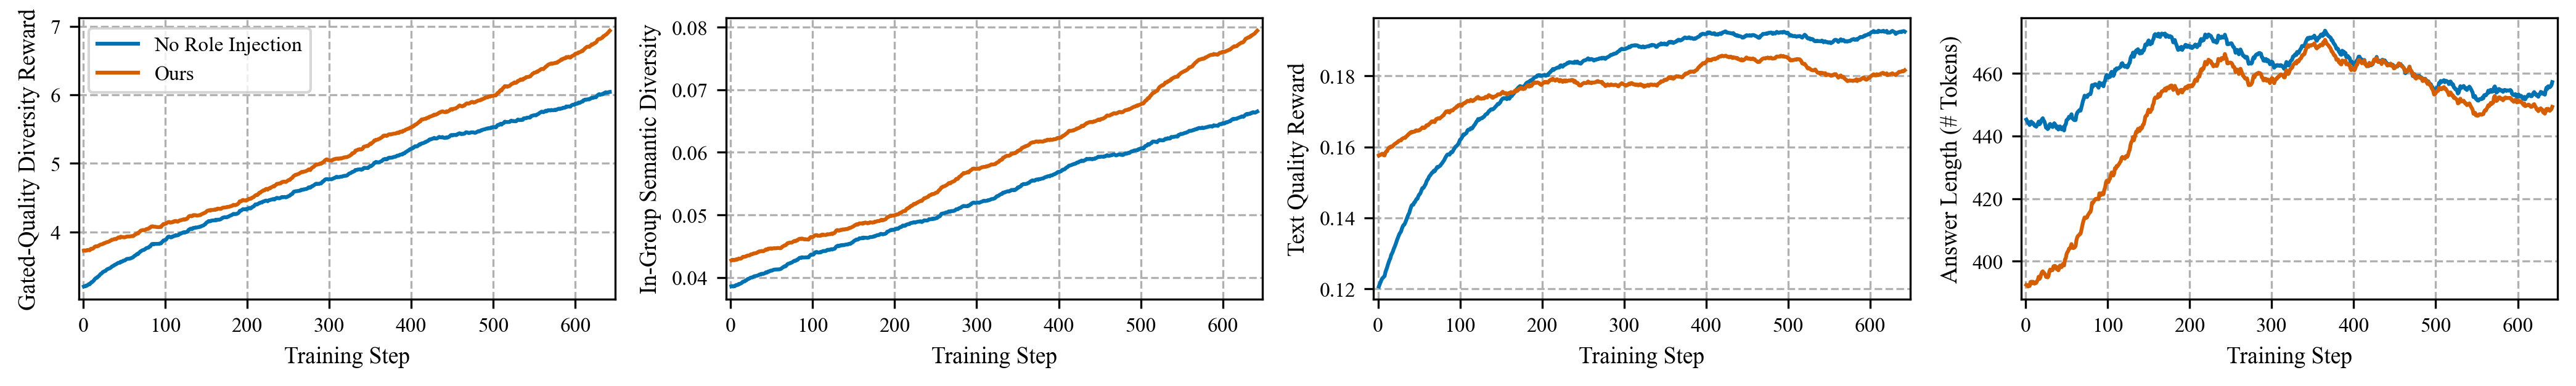
\includegraphics[width=0.82\linewidth]{figures/no_role_wo.png}
    \end{subfigure}
    \caption*{\textbf{No role injection, thinking disabled.}}

    \begin{subfigure}{\textwidth}
        \centering
        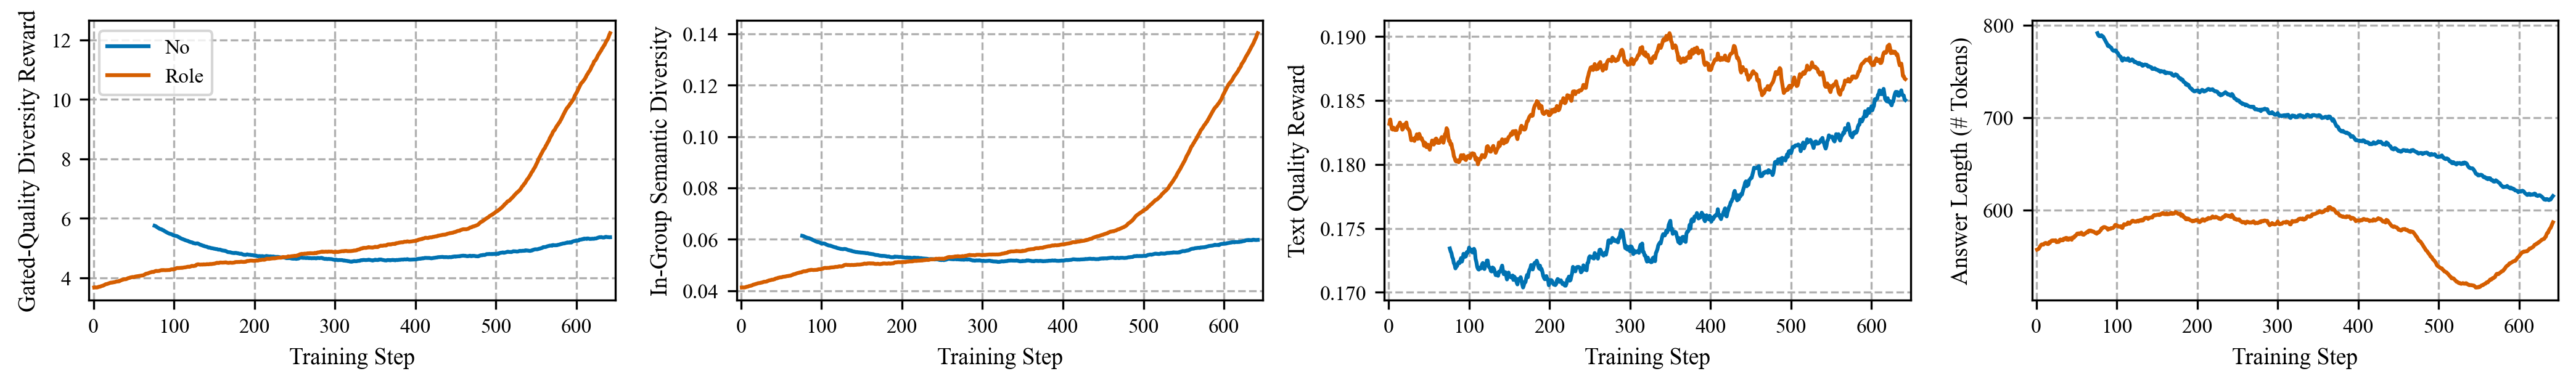
\includegraphics[width=0.82\linewidth]{figures/no_role_w.png}
    \end{subfigure}
    \caption*{\textbf{No role injection, thinking enabled.}}

    \vspace{0.7em}
    % Row 3: Quality-only, thinking disabled
    \begin{subfigure}{\textwidth}
        \centering
        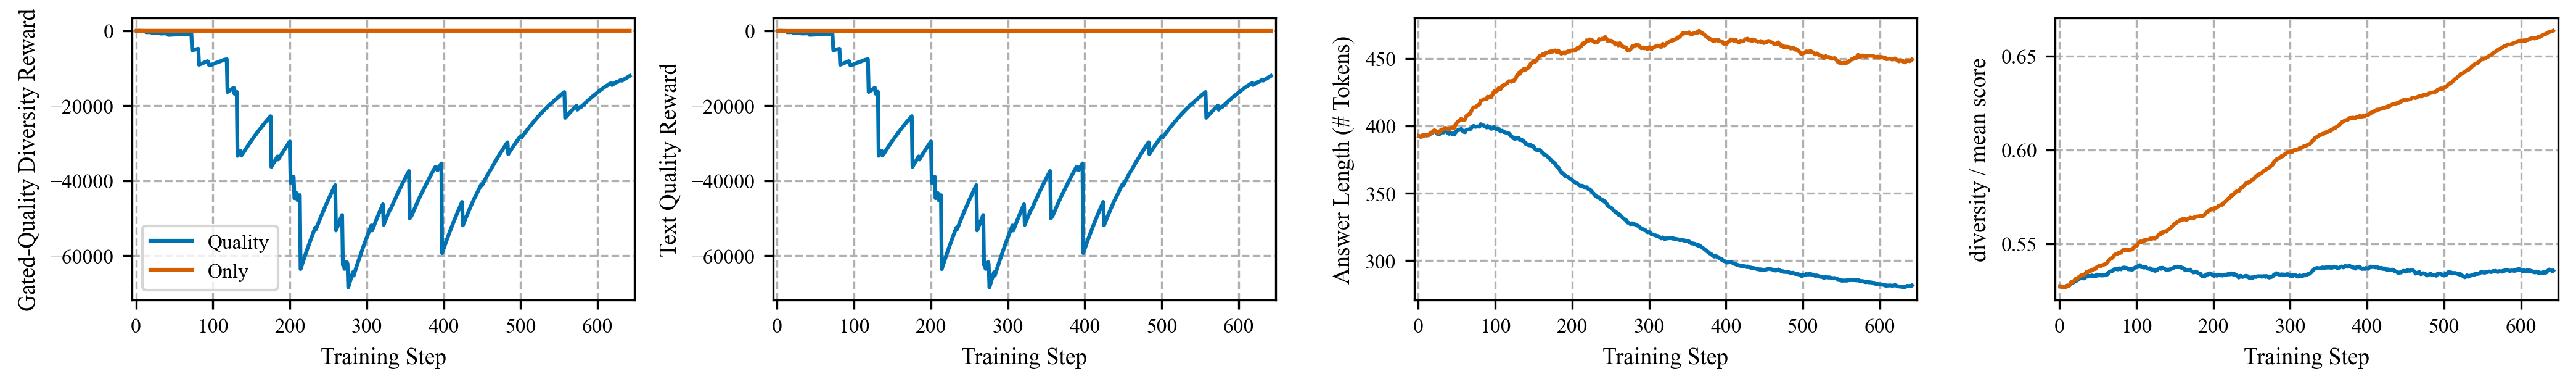
\includegraphics[width=0.82\linewidth]{figures/quality_only_wo.png}
    \end{subfigure}
    \caption*{\textbf{Quality-only reward, thinking disabled.}}

    \vspace{0.7em}

    % Row 4: Quality-only, thinking enabled
    \begin{subfigure}{\textwidth}
        \centering
        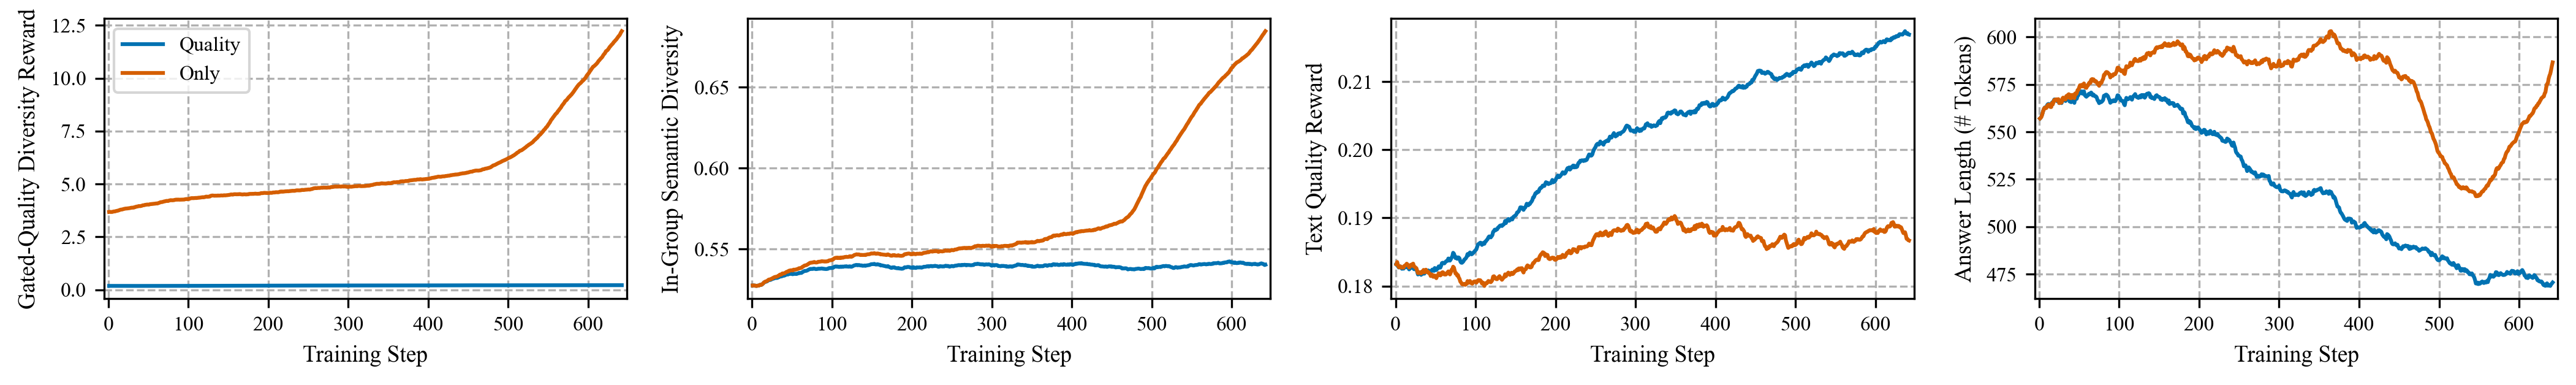
\includegraphics[width=0.82\linewidth]{figures/quality_only_w.png}
    \end{subfigure}
    \caption*{\textbf{Quality-only reward, thinking enabled.}}

     \vspace{0.7em}
    % Row 3: Diversity-only, thinking disabled
    \begin{subfigure}{\textwidth}
        \centering
        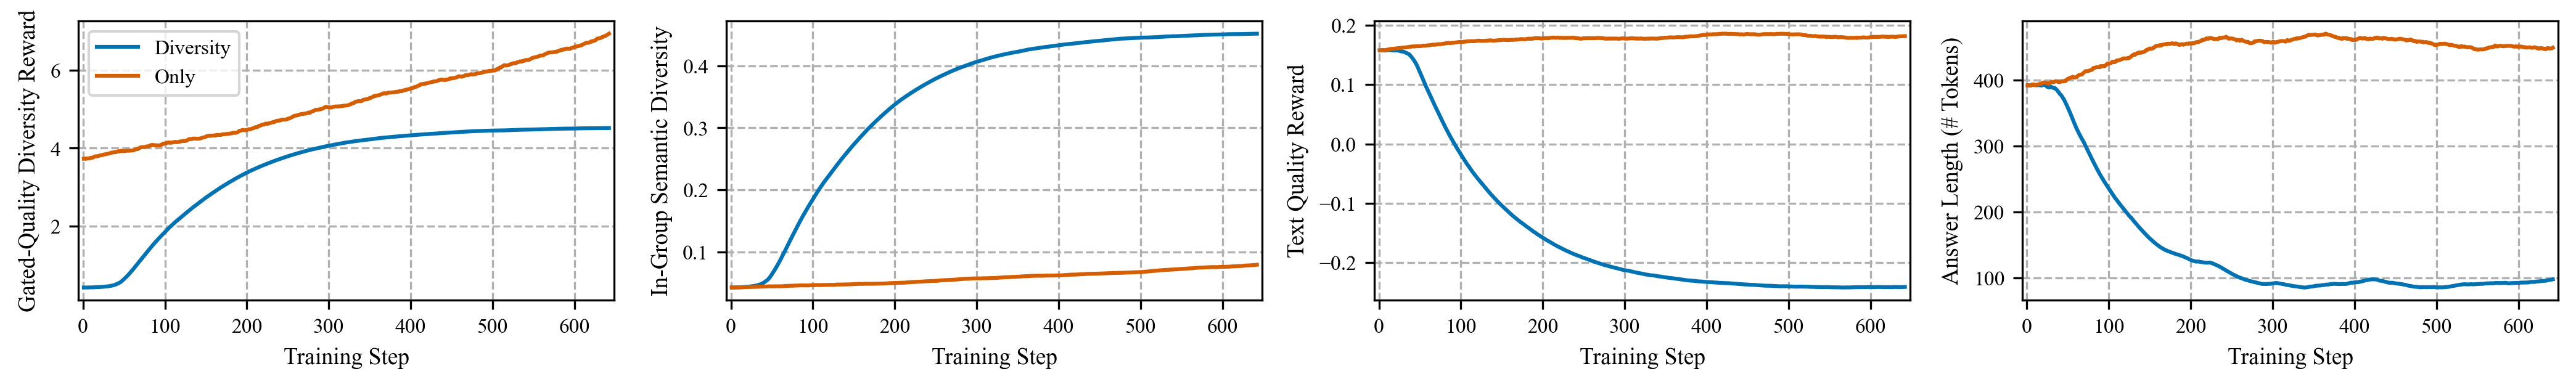
\includegraphics[width=0.82\linewidth]{figures/diversity_only_wo.png}
    \end{subfigure}
    \caption*{\textbf{Diversity-only reward, thinking disabled.}}

    \vspace{0.7em}

    % Row 4: Diversity-only, thinking enabled
    \begin{subfigure}{\textwidth}
        \centering
        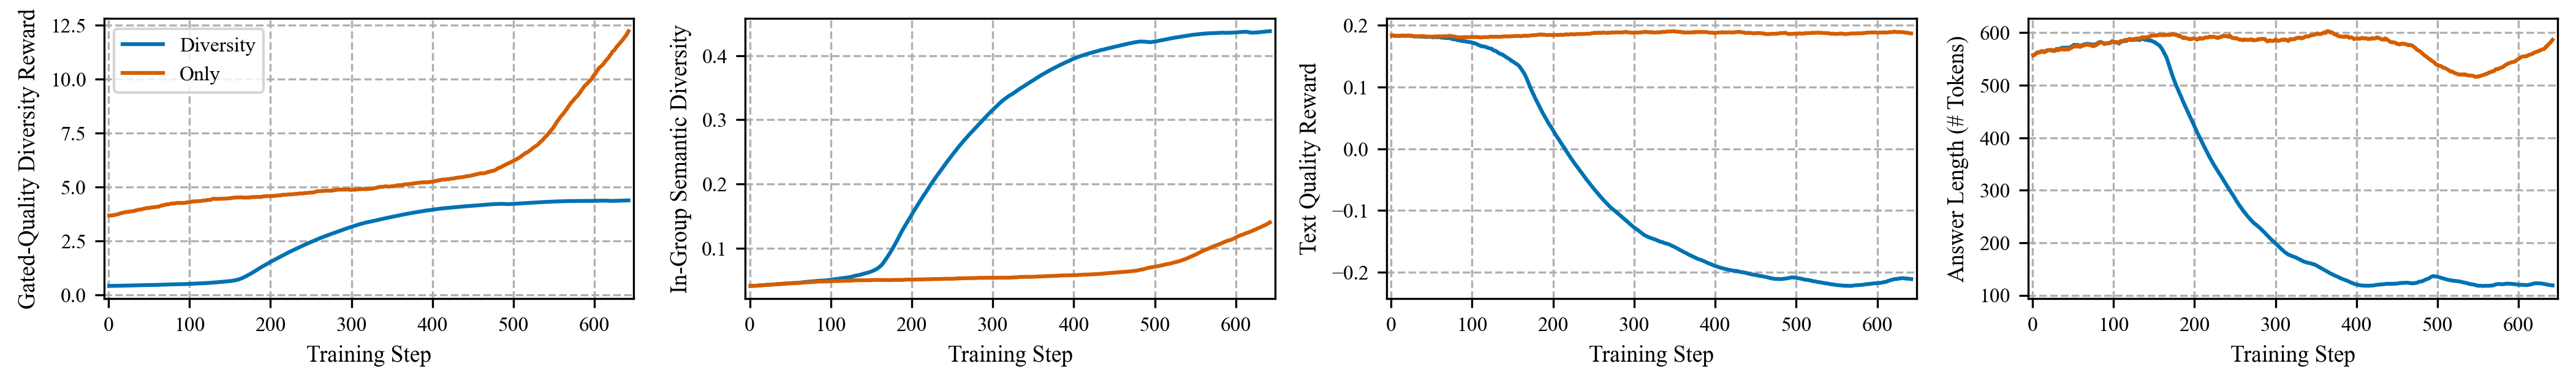
\includegraphics[width=0.82\linewidth]{figures/diversity_only_w.png}
    \end{subfigure}

    \caption*{\textbf{Diversity-only reward, thinking enabled.}}

    % Row 3: Crafted role, thinking disabled
    \begin{subfigure}{\textwidth}
        \centering
        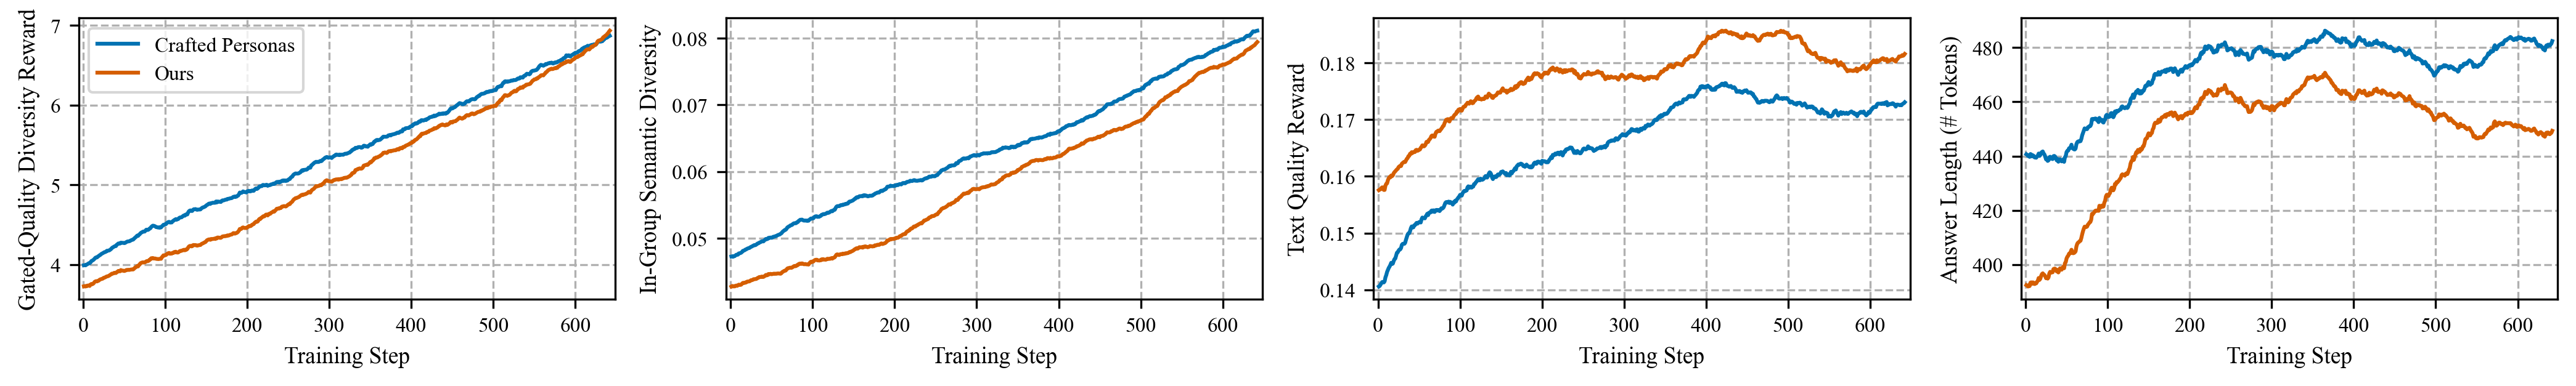
\includegraphics[width=0.82\linewidth]{figures/crafted_wo.png}
    \end{subfigure}
    \caption*{\textbf{Crafted personas, thinking disabled.}}

    \vspace{0.7em}

    % Row 4: Crafted role, thinking enabled
    \begin{subfigure}{\textwidth}
        \centering
        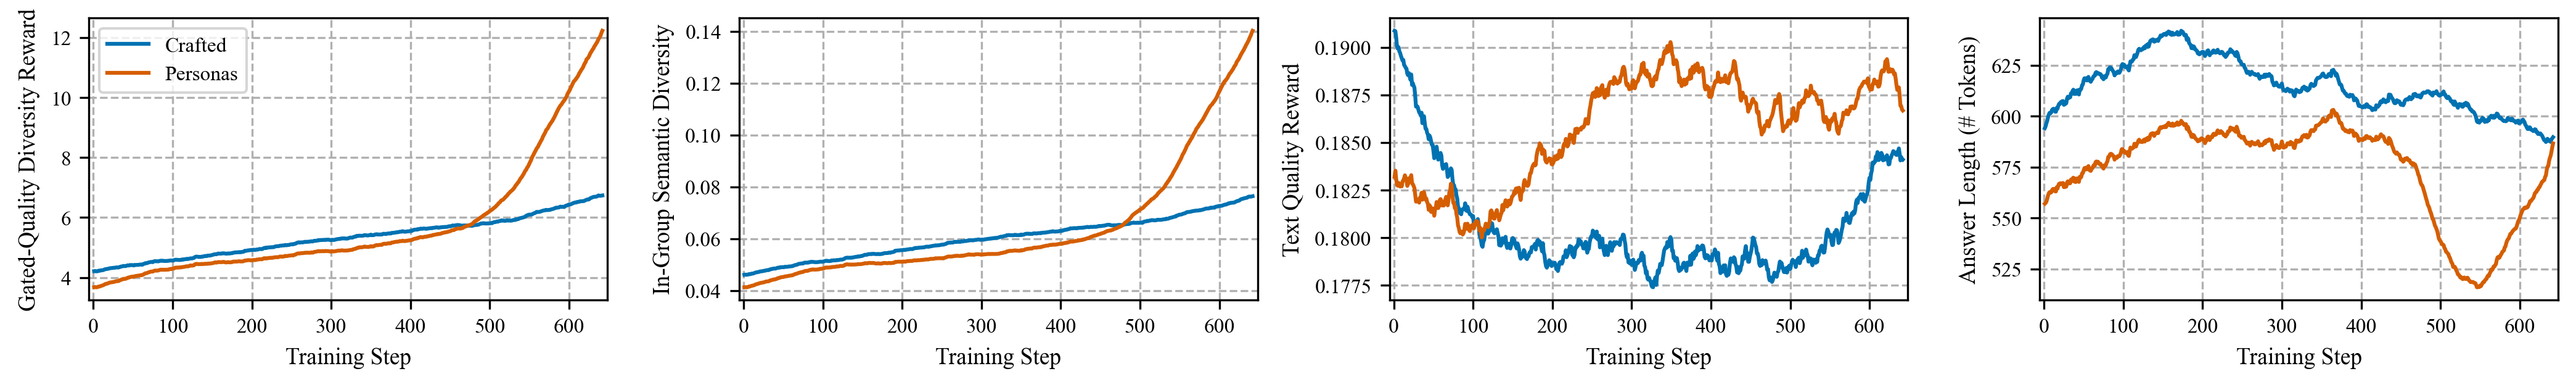
\includegraphics[width=0.82\linewidth]{figures/crafted_w.png}
    \end{subfigure}
    \caption*{\textbf{Crafted personas, thinking enabled.}}



    \caption{
    Training curves for ablation studies. Each row corresponds to one ablation setting, and each row reports four training diagnostics: total reward, diversity reward, quality reward, and answer token length. Results are shown under both thinking-disabled and thinking-enabled settings.}
    \label{fig:ablation-training-curves}
\end{figure}

